\documentclass{article}
\usepackage{amsmath, amsthm, amsfonts}
\usepackage{bm}
\usepackage{graphicx}
\usepackage{xcolor, soul}  
\usepackage{mathtools}
\usepackage{parskip}

\title{CSC301 Lecture 10}
\author{1910456 Mir Shafayat Ahmed}
\color{black}
\begin{document}
    \pagecolor[HTML]{FFFFCC}
    \maketitle
    \subsection*{Regex to CFG}
    We use the following replacements when converting different operations in regex to CFG.
    $$\emptyset = grammar\;with\;no\;rules$$
    $$\varepsilon = G\to\varepsilon$$
    $$A^*= G\to GA\;|\;\varepsilon$$
    $$A+B = G\to A\;|\;B$$
    $$AB = G\to AB$$
    So, to convert (0+1)*111,
    We can divide it into two parts, one with the ()* and one with the 111 and use the other replacements to find,
    $$S\to N111$$
    $$N\to N0\;|\;N1\;|\;\varepsilon$$


    \section*{Ambiguity}
    If a string has more than one parse tree, we call the CFG ambiguous. Such as for the string 1+2*2, without the parenthesis, the CFG would be ambiguous.\par
    For a CFG that has a rule $N\to NN$  compared to a rule that says $N\to DN$, there is ambiguity on where to add the next sequence. (To add to the left or to the right).\par
    $$S\to SS\;|\;x$$
    \begin{figure}[h]
        \centerline{
            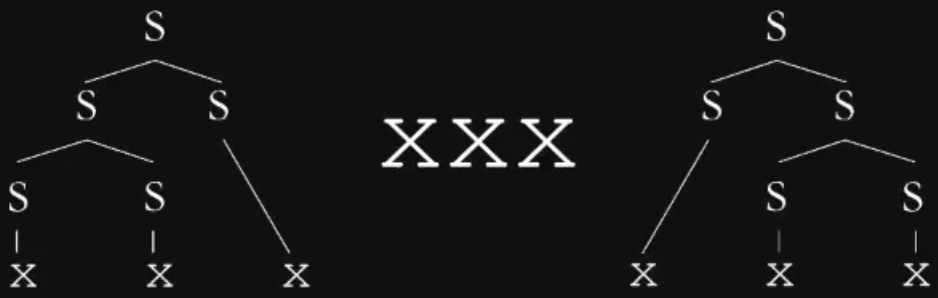
\includegraphics[scale=0.20]{Ambiguity.png}
        }\caption{Different parse tree for same string}
        \label{ambiguity}
    \end{figure}
    \\
    But we can fix CFG of Figure \ref{ambiguity} by simply changing it to
    $$S\to Sx\;|\;x$$
    And now, subsequent additions tot the tree  can only take one path.
    \begin{figure}[h]
        \centerline{
            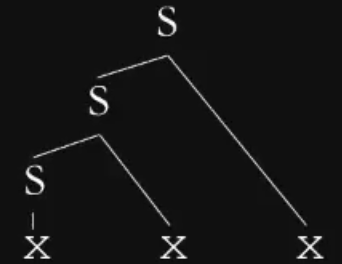
\includegraphics[scale=0.25]{AmbiguityFix.png}
        }\label{ambiguityfix}
        \caption{New Unique Parse Tree}
    \end{figure}    
    \subsection*{Disambiguation}
    When we are looking to make a language unambiguous, we might not succeed as some languages are inherently unambiguous. Also, there is no general procedure tot follow.\par
    In programming languages, ambiguity comes from not using parenthesis. In spoken languages as well, there can be some ambiguity.

    \begin{quote}
        "She fixed the light on the top floor"
    \end{quote}
    
    \subsection*{Parsing}
    For the CFG,
    $$S\to 0S1\;|\;1S0S\;|\;T$$
    $$T\to S\;|\;\varepsilon$$
    If we want to build a parse tree for the string '0011', we can go on and on without any final destination.\par
    It is because of a few reasons,
    \begin{itemize}{}{}
        \item The string might not be in the language and so we are on a never-ending search.
        \item For longer strings, the permutation of parse trees would be too many.
    \end{itemize}
    We therefore have an idea to:\par
    \textbf{Stop when the length of a derived string exceeds the required string}\par
    But here we encounter two problems:
    \begin{enumerate}
        \item Due to empty transitions, strings containing Variables may turn into empty strings and reduce the length of the string later on.
        \item Rules that have Unit transitions like $A\to B$ may continue looping forever.
    \end{enumerate}
    So, to resolve the two issues, we modify our CFG so that there are no $\varepsilon$ and unit productions. After which, \textbf{we can be sure that any derivation can only grow the string and not shrink or remain constant in length}.
    
    \subsection*{Removing $\bm{\varepsilon}$-productions}
    If the start variable is nullable,
    $$S\to \varepsilon$$
    we add a new start variable $S'$ and add a new production,
    $$S'\to S\;|\;\varepsilon$$\par 
    For other nullable variables,
    \begin{enumerate}
        \item We identify a nullable variable and remove the $\varepsilon$-production
        \item We look for references of that variable in other productions and replace that reference with what would've happened if the nullable variable wasn't removed.
    \end{enumerate}
    
    \subsubsection*{Example}
    For the CFG,
    \begin{equation}
        \begin{split}
            S&\to ACD\\
            A&\to a\\
            B&\to \varepsilon\\
            C&\to ED\;|\;\varepsilon\\
            D&\to BC\;|\;b\\
            E&\to b\\
        \end{split}
    \end{equation}
    We identify B as a nullable variable, so we remove $B\to\varepsilon$.
    Now we look for references and see that B is referenced in $D\to BC$. So we replace B with what it was supposed to be, i.e 'empty'. And so, we get,
    \begin{equation}
        \begin{split}
            S&\to ACD\\
            A&\to a\\
            C&\to ED\;|\;\varepsilon\\
            D&\to C\;|\;b\\
            E&\to b\\
        \end{split}
    \end{equation} 
    Now we look for more nullable variables and see that C is nullable. So we remove $C\to\varepsilon$. 
    We see that C is referenced in the beginning. so we change it to $S\to AD$. But, now we cannot form something like 'AEDD' that was possible before, therefore we keep $S\to ACD$ as well.\\
    D also references C, so we replace it with $D\to\varepsilon$. But again, D could be ED before, so we keep $D\to C$
    \begin{equation}
        \begin{split}
            S&\to ACD\\
            S&\to AD\\
            A&\to a\\
            C&\to ED\\
            D&\to C\;|\;b\;|\;\varepsilon\\
            E&\to b\\
        \end{split}
    \end{equation}
    We repeat and remove $D\to\varepsilon$.
    Now $S\to ACD$ can be $S\to AC$ as well. For the other reference, the same logic applies and we end up with,
    \begin{equation}
        \begin{split}
            S&\to ACD\;|\;AC\\
            S&\to AD\;|\;A\\
            A&\to a\\
            C&\to ED\;|\;E\\
            D&\to C\;|\;b\\
            E&\to b\\
        \end{split}
    \end{equation}
    Finally we see that there aren't any nullable variables anymore. So we have solved our first problem regarding disambiguation.


\end{document}